\documentclass{anstrans}
%%%%%%%%%%%%%%%%%%%%%%%%%%%%%%%%%%%
\title{Online reprocessing simulation for thorium-fueled molten salt breeder reactor}

\author{Andrei Rykhlevskii, Alexander Lindsay, Kathryn Huff}

\institute{
Department of Nuclear, Plasma, and Radiological Engineering, University of Illinois at Urbana-Champaign \break
Urbana, IL
}

\email{andreir2@illinois.edu}

%%%% packages and definitions (optional)
\usepackage{graphicx} % allows inclusion of graphics
\usepackage{caption}  % allows center figures caption
\usepackage{booktabs} % nice rules (thick lines) for tables
\usepackage{microtype} % improves typography for PDF
\usepackage[section]{placeins}

\usepackage[acronym,toc]{glossaries}  % acronyms inclusion
\include{acros}
	
\makeglossaries

\graphicspath{{figures/}}

\newcommand{\SN}{S$_N$}
\renewcommand{\vec}[1]{\bm{#1}} %vector is bold italic
\newcommand{\vd}{\bm{\cdot}} % slightly bold vector dot
\newcommand{\grad}{\vec{\nabla}} % gradient
\newcommand{\ud}{\mathop{}\!\mathrm{d}} % upright derivative symbol

\begin{document}
%%%%%%%%%%%%%%%%%%%%%%%%%%%%%%%%%%%%%%%%%%%%%%%%%%%%%%%%%%%%%%%%%%%%%%%%%%%%%%%%
\section{Introduction}
The thermal spectrum \gls{MSR} is an advanced type of reactor consist of constantly circulating liquid fuel (i.e., mixture of $LiF-BeF_2-ThF_4-UF_4$ or $LiF-BeF_2-ZrF_4-UF_4$) which works also as a coolant, and the reactor graphite as moderator. This fuel form leads to immediate advantages over traditional, solid-fueled, reactors. The molten-salt carrier salt with dissolved in it fissile and/or fertile material allows to use online refuelling and reprocessing, which means \gls{MSR}s can operate years without shutdown, achieve maximum fuel utilization, and outstanding neutron economy \cite{leblanc_molten_2010}. Moreover, this type of fuel does not need fabrication and could be transported from enrichment plant to \gls{NPP} in form of uranium hexafluoride ($UF_6$), so \gls{MSR}s are also beneficial with regards to economics. Additionally, it has high level of inherent safety due to strong negative temeperature coefficient of reactivity, near-atmospheric pressure in the primary loop, stable coolant, passive decay heat cooling, and small excess reactivity \cite{elsheikh_safety_2013}.

The thorium fueled \gls{MSBR} was developed in early 1970s by \gls{ORNL} specifically to realize the promise of the thorium fuel cycle which allows the use of natural thorium instead of enriched uranium as the fertile element. Thorium breeds the fissile $^{233}U$ and avoids uranium enrichment \cite{robertson_conceptual_1971}. In the matter of nuclear fuel cycle, the thorium cycle produces much less amount of plutonium and minor actinides (MAs) comparing to the traditional uranium fuel cycle, consequently, it might significantly increase prolifiration resistance when \gls{MSR} operates in the breeder regime. The \gls{MSR}s also could be employed as converter reactor for transmutation spent fuel from \gls{LWR} or others.

Nowadays, interest to \gls{MSR} coming back after long-term break because of its unique characteristics and features of this type of reactor, such as online reprocessing and refueling. For the development of \gls{MSR} conception special computational analysis methods and codes needed due to completely different physics of liquid-fueled nuclear reactor comparing with traditional, solid-fueled, reactors. Most of the contemporary nuclear reactor physics codes do not able to perform depletion calculations in the online reprocessing regime. J.J. Powers (\gls{ORNL}) has suggested a novel method to conducting depletion simulation for \gls{MSR} with taking into account the online reprocessing and refueling based on the deterministic computer code NEWT in SCALE \cite{powers_new_2013}. This approach was later used by Jeong et al. to find equilibrium state for \gls{MSBR} and validate it with \gls{MCNP}/CINDER90 model \cite{jeong_equilibrium_2016}. For the development of \gls{MSBR} research, this paper presents the single-cell model developed using a continuous-energy the Serpent 2 Monte Carlo reactor physics calculation code that was employed to find equilibrium core state, and several calculation results including the depletion calculation of the single-cell unit.

All calculations presented in this paper were performed using the Serpent 2 code version 2.1.29 with ENDF/B-VII
nuclear data \cite{leppanen_serpent_2012,chadwick_endf/b-vii.0:_2006}. Compared to Serpent 1, Serpent 2 has many more useful features and contains a complete redesign of memory management using hybrid OpenMP + MPI parallelization, which is important in depletion calculations using computer clusters with multiple cores \cite{leppanen_serpent_2015}. This paper use build-in Serpent 2 depletion capabilities with online reprocessing subroutine. Another feature of \gls{MSBR}, circulating
liquid fuel, which causes delayed neutron precursor drift is not treated here.

%%%%%%%%%%%%%%%%%%%%%%%%%%%%%%%%%%%%%%%%%%%%%%%%%%%%%%%%%%%%%%%%%%%%%%%%%%%%%%%%
\section{Description of the actual work}
The \gls{MSBR} is thermal spectrum reactor. The reactor vessel has diameter of 680 cm and a height of 610 cm and contains molten fluoride fuel-salt mixture which performs two functions: to generate heat in the moderated region and to transport heat energy from the core to primary heat exchanger using the primary salt pump. The vessel also contains graphite blocks for neutron moderation and reflection. The lithium in the fuel-salt solution is enriched to 99.995\% $^7$Li because $^6$Li is a very strong neutron poison and becomes tritium upon neutron bombardment. In this study, the 0.005\% atomic fraction of $^6$Li has been taken into account because even such a small amount of isotope with very high absorption cross section might significantly affect on neutron flux energy distribution and, consequently, on depletion calculation results. Table~\ref{tab:data} is the summary of the major \gls{MSBR} parameters \cite{robertson_conceptual_1971}. 

%%%%%%%%%%%%%%%%%%%%%%%%%%%%%%%%%%%%%%%%
\captionsetup[table]{
  labelsep = newline,
  name = TABLE, 
  justification=justified,
  singlelinecheck=false,%%%%%%% a single line is centered by default
  labelsep=colon,%%%%%%
  skip = \medskipamount}
\begin{table}[h!]
%\centering
\begin{tabular}{p{0.46\linewidth} p{0.50\linewidth}} \toprule
Thermal capacity of reactor           & 2250 MW(t)
\\ \midrule
%Net electrical output                 & 1000 MW(e) 
%\\ \midrule
%Net thermal efficiency        & 44.4\%
%\\ \midrule
Volume fraction of salt in central core zone     & 0.132
\\ \midrule
Volume fraction of salt in outer core zone       & 0.37
\\ \midrule
Fuel-salt inventory (Zone I)                  & 8.2 m$^3$	
\\ \midrule
Fuel-salt inventory (Zone II)                 & 10.8 m$^3$	
\\ \midrule
Fuel salt components                  & LiF-BeF$_2$-ThF$_4$-$^{233}$UF$_4$-$^{239}$PuF$_3$	
\\ \midrule
Fuel salt composition                 & 71.767-16-12-0.232-0.0006 mole\%
\\
\bottomrule
\end{tabular}
  \caption{Summary of principal data for MSBR.}
  \label{tab:data}
\end{table}
%%%%%%%%%%%%%%%%%%%%%%%%%%%%%%%%%%%%%%%%%%%%%%%%

The \gls{MSBR} core consist of two different zones with one flow. The central zone, Zone I, in which 13.2\% of the volume is fuel salt and 86.8\% graphite. The first zone is composed of 1320 graphite cells, 2 graphite control rods, and 2 safety rods consisting of boron carbide clad. The undermoderated zone, Zone II, with 37\% fuel salt, and radial reflector, surrounding the more active portion serves to diminish neutron leakage from the reactor core. In this work, only Zone I element with the hole diameter of 3.42138 cm, and the molten-salt fuel volume fraction is 0.132 was considered. Figure~\ref{fig:zoneI} shows the geometry of unit cell model. The boundary condition of the unit cell is periodic. The density of fuel salt is 3.3304 g/cm$^3$ and graphite one is 1.843 g/cm$^3$. The temperature of fuel and graphite is fixed for the whole reprocessing cycle at 908K \cite{robertson_conceptual_1971}.

\begin{figure}[h] % replace 't' with 'b' to force it to be on the bottom
  \centering
  \vspace{-0.6em}
  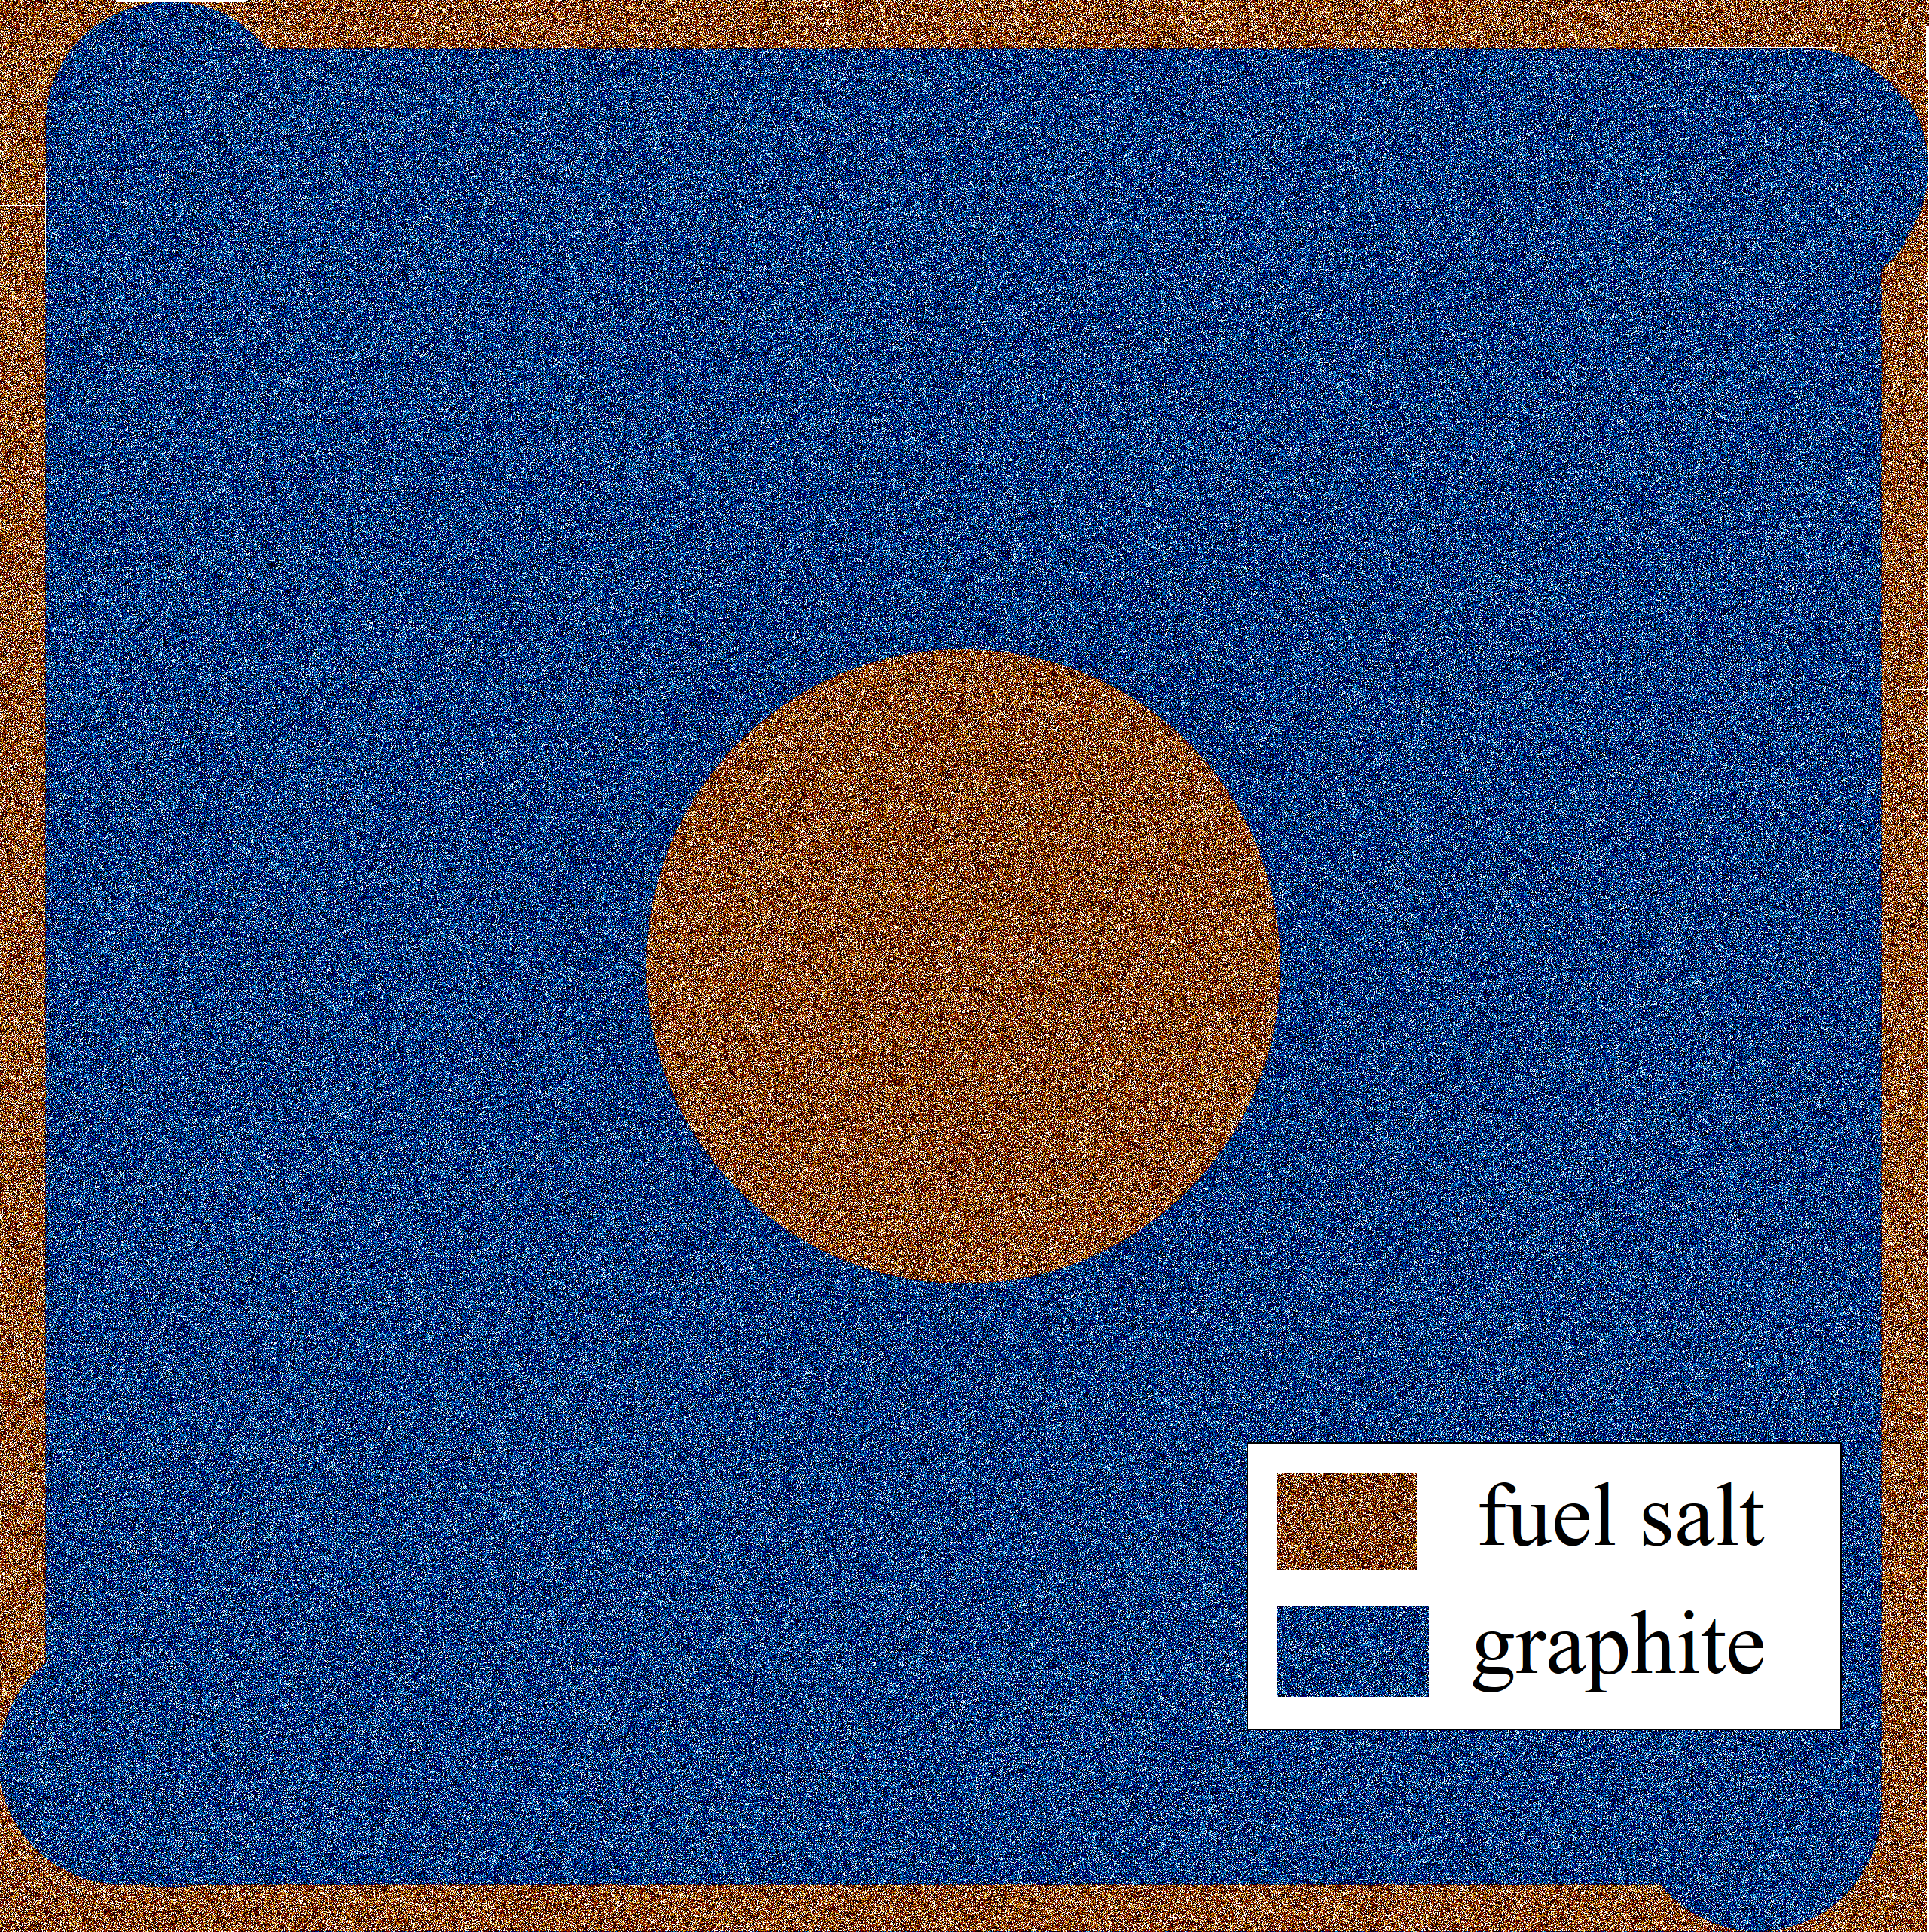
\includegraphics[width=0.99\linewidth]{zone_I_mesh.png}
  \caption{MSBR unit cell of Zone I geometry.}
  \label{fig:zoneI}
\end{figure}
\subsection{Online reprocessing method}

Currently, researchers usually using supporting tools and scripts to simulate online reprocessing and refueling. Most researchers investigating the \gls{MSR}s have utilised for reprocessing calculations stochastic (i.e. \gls{MCNP}) or deterministic (i.e. SCALE) code with originally-developed scripts based on Python \cite{jeong_equilibrium_2016,park_whole_2015}. The Serpent 2 is the first code supporting continuous material reprocessing, and allows create needed number of material flows into the fuel and/or out from the fuel.

The \gls{MSBR} has the capability to remove every 20 seconds all poisons (e.g. $^{135}$Xe), noble metals and gases (e.g. $^{75}$Se, $^{85}$Kr) which also have relatively high absorption cross section. The thorium-232 absorbs thermal neutrons and produce $^{233}$Pa which then decay into the fissile $^{233}$U. The problem of protactinium is a large absorption cross section in the thermal energy spectrum, therefore $^{233}$Pa continuously removing from fuel salt into protactinium decay tank and allowing $^{233}$Pa to decay to $^{233}$U without reactor poisoning. The reactor reprocessing system designed to separate $^{233}$Pa from the molten-salt fuel over 3 days, held it to produce $^{233}$U and return it back to the primary loop. This feature allows to keep the neutrons losses to protactinium and fission products to a very low level, and increses the efficency of $^{233}$U breeding \cite{robertson_conceptual_1971}.

A major problem with the reprocessing method is that different nuclides have specific removal rates. On the one hand, if the depletion time intervals are very short it means specific isotope beign instantly removed, and it is hard to obtain equilibrium composition because enormous large number of depletion steps. On the other hand, if the depletion calculation time interval is too long the results would not truly represents \gls{MSBR} conceptual design. Following this idea, the time interval for depletion calculations was selected 3 days that correlate with the removal interval of $^{233}$Pa which is the major isotope for producing $^{233}$U. Thorium is continuously adding to maintain the initial mass fraction of $^{232}$ThF$_4$.

%%%%%%%%%%%%%%%%%%%%%%%%%%%%%%%%%%%%%%%%%%%%%%%%%%%%%%%%%%%%%%%%%%%%%%%%%%%%%%%%
\section{Results and Analysis}

Using the methodology described previously, the \gls{MSBR} unit cell depletion analysis was performed to find equilibrium core conditions. In this section, the calculation results including multiplication factor, neutron flux energy spectrum, atomic density of major isotopes are summarised.

\subsection{Temperature effect of reactivity}
Table~\ref{tab:tcoef} represents the quantitive analysis of temperature effects on reactivity. Uncertainty for each temperature coefficient also was calculated and shown in Table~\ref{tab:tcoef}. The main physical principle underlying the reactor temperature feedback is expandsion of matter when it is heated. When the fuel salt temperature increases, the density of the salt decreases, but at the same time, the total volume of fuel salt in the core remains constant because it is defined by the space for fuel bounded by the graphite. When the reactor graphite temperature grows, the density of graphite declines which also frees up space for fuel salt. To determine temperature coefficients, three cases were considered:
\begin{enumerate}  
\item Temperature of fuel salt rising from 900K to 1200K.
\item Temperature of graphite rising from 900K to 1200K. 
\item Whole reactor temperature rising from 900K to 1200K.
\end{enumerate}

%%%%%%%%%%%%%%%%%%%%%%%%%%%%%%%%%%%%%%%%
\captionsetup[table]{
  labelsep = newline,
  name = TABLE, 
  justification=justified,
  singlelinecheck=false,%%%%%%% a single line is centered by default
  labelsep=colon,%%%%%%
  skip = \medskipamount}
\begin{table}[h!]
%\centering
\begin{tabular}{p{0.22\linewidth} p{0.22\linewidth} p{0.21\linewidth} p{0.15\linewidth}} \toprule
   Reactivity coefficient [pcm/K]  & Serpent2      & MCNP6 \cite{park_whole_2015}   & Reference \cite{robertson_conceptual_1971}      
\\ \midrule
Fuel salt        & $-3.93\pm0.005$ & $-3.20\pm0.05$ & $-3.22$ 
\\ \midrule
Moderator        & $+2.44\pm0.013$ & $-0.11\pm0.05$ & $+2.35$ 
\\ \midrule
Total            & $-1.74\pm0.030$ & $-3.21\pm0.04$ & $-0.87$ 
\\
\bottomrule
\end{tabular}
  \caption{Temperature coefficients of reactivity.}
  \label{tab:tcoef}
\end{table}
%%%%%%%%%%%%%%%%%%%%%%%%%%%%%%%%%%%%%%%%%%%%%%%%%%%%%%%%%%%%%%%%%%%%%%%%%%%%%%%%
On the one hand, changes in fuel temperature cause only density variation, geometry keeps the same because fuel is in the form of liquid. On the other hand, when moderator heats up both the density and the geometry changes due to thermal expansion of the graphite blocks and the reflector. New graphite density was calculated using linear temperature expansion coefficient of reactor graphite which is $1.3\times10^{-6}1/K$ \cite{robertson_conceptual_1971}. Based on this information new geometry input, which takes into account graphite expansion, was created.

The fuel temperature coefficient (FTC) is positive due to thermal Doppler broadening of the resonance capture cross sections in the thorium and is in a good agreement with early research \cite{robertson_conceptual_1971,park_whole_2015}. The moderator temperature coefficient is negative due to changing density, and would increases during reactor operation because of spectrum hardening along with fuel depletion \cite{park_whole_2015}. Finally, the total temperature coefficient of reactivity is relatively large and negative, despite graphite components, and affords excellent reactor stability and controllability.
%%%%%%%%%%%%%%%%%%%%%%%%%%%%%%%%%%%%%%%%%%%%%%%%%%%%%%%%%%%%%%%%%%%%%%%%%%%%%%%%
\section{Conclusions}
The MSBR full-core analysis was performed using the Serpent 2 Monte Carlo code. The complex geometry of the reactor is reconstructed in three-dimensional space without any major approximations. Accurate material data was employed to calculate reactor key design parameters. The effective multiplication factor for initial fuel composition is slightly higher than 1 (1.05) which allows reactor operation from startup to first online reprocessing cycle. The neutron flux energy spectrum was calculated for the whole core and represents the epithermal spectrum of the MSBR. The total temperature coefficient is negative, consequently, the MSBR has negative temperature feedback, but MTC is negative which has a negligible effect on safety because it is outweighed by the strong, negative FTC.

This high-fidelity full-core model will be employed for a number of future efforts. First, depletion simulation will be performed using built-in Serpent 2 depletion capabilities to find the equilibrium state of the MSBR, its optimal fuel salt composition, reprocessing characteristics (i.e. rates of removing fission products, the rate of adding thorium), and fuel utilization. Secondly, the model will be used to generate problem-oriented nuclear data libraries for multi-physics models of MSRs developed in the MOOSE-based coupled neutronics/thermal-hydraulics code Moltres \cite{lindsay_arfc/moltres:_2017}. Finally, transient accident simulations for safety investigation of the reactor core will be performed to study the dynamic behavior of Molten Salt Breeder Reactor. 


%%%%%%%%%%%%%%%%%%%%%%%%%%%%%%%%%%%%%%%%%%%%%%%%%%%%%%%%%%%%%%%%%%%%%%%%%%%%%%%%
\bibliographystyle{ans}
\bibliography{bibliography}
\end{document}

